\documentclass{beamer}
\usepackage{xypic}
\usepackage{amsmath}
\usepackage{amssymb}
\usepackage{amsthm, bbm}
\usepackage{graphicx}
\graphicspath{{./figs/}}
\usepackage{tikz}

%Shortcuts
\newcommand{\cc}{\mathbb{C}}
\newcommand{\zz}{\mathbb{Z}}
\newcommand{\rr}{\mathbb{R}}
\renewcommand{\sl}{\text{sl}}
\newcommand{\tb}{\text{tb}}
\newcommand{\lk}{\text{lk}}
\newcommand{\st}{{\text{st}}}
\newcommand{\id}{\operatorname{id}}
\newcommand{\pr}{\operatorname{pr}}
\newcommand{\Symp}{\operatorname{Symp}}
\newcommand{\Mod}{\operatorname{Mod}}
\newcommand{\Diff}{\operatorname{Diff}}
\newcommand{\km}{{\normalfont{(KM)}}}
\newcommand{\vol}{\operatorname{vol}}
\newcommand{\defeq}{\mathrel{\vcenter{\baselineskip0.5ex\lineskiplimit0pt\hbox{\scriptsize.}\hbox{\scriptsize.}}}=}
\newcommand{\hs}{\hspace{0.05em}} % half-space


%Environments
\newtheoremstyle{thm}{15 pt}{10 pt}{\itshape}{}{\bfseries}{.}{.5em}{}
\newtheorem{thm-main}{Theorem}
\newtheorem{conjecture}[theorem]{Conjecture}
\newtheorem{proposition}[theorem]{Proposition}
\newtheorem*{thm*}{Theorem}
\newtheorem*{cor*}{Corollary}

\newtheoremstyle{ex}{10 pt}{10 pt}{\normalfont}{}{\bfseries}{.}{.5em}{}
\theoremstyle{ex}

\newtheoremstyle{rem}{10 pt}{10 pt}{\normalfont}{}{\it}{.}{.5em}{}
\theoremstyle{rem}
\newtheorem{remark}[theorem]{Remark}


\title[Integer Characterizing Slopes]{Knot Surgery and Integer Characterizing Slopes}
\usetheme{Madrid}

\author[Agostini, Chen, Serio, Wang, Wu, and Wu\;\;\;]{Gabriel Agostini, Sophia Chen, Christian Serio, Cecilia Wang, Anton Wu, and Kexin Wu\\
Advisors: Kyle Hayden and Aliakbar Daemi}
\institute{Columbia University}
\date{August 1, 2019}

\begin{document}
	
	\begin{frame}
		\titlepage
	\end{frame}

	\begin{frame}
		\frametitle{Knots and links in the 3-sphere}
		\begin{definition}
			A \textit{knot} $K$ is the image of a smooth embedding of the circle $S^1$ into a 3-manifold, usually the $3$-sphere $S^3$. In particular, $K$ is diffeomorphic to $S^1$. A \textit{link} $L$ is a disjoint union of knots, which may be knotted together.
		\end{definition}
		\begin{definition}
		Let $M,N$ be manifolds and $g,h\!:N\to M$ embeddings. An \textit{ambient isotopy} of $M$ carrying $g$ to $h$ is a continuous map $F\!:M\times[0,1]\to M$, such that $F_t=F(\cdot,t)$ is a homeomorphism of $M$ for each $t\in[0,1]$,  $F_0=\mathbbm{1}$, and $F_1\circ g = h$.
		\end{definition}
		\begin{itemize}
		\item We regard two knots $K,K'\subset S^3$ to be equivalent if they differ by an ambient isotopy of $S^3$. We write $K\simeq K'$.	
		\item Equivalently, we can view knots as subsets of $\mathbb{R}^3$ rather than $S^3$.
		
		\end{itemize}
	\end{frame}

	\begin{frame}
		\frametitle{Knot diagrams}
		\begin{itemize}
			\item We can study a knot $K\subset\mathbb{R}^3$ by projecting it onto a hyperplane $\mathbb{R}^2$.
			
			\item If $\pi\!:\mathbb{R}^3\to\mathbb{R}^2$ is a projection such that $\pi(K)$ is an embedded curve except at finitely many \textit{crossing points}, then $\pi(K)$ is a \textit{diagram} for $K$.
			
			\item The \textit{crossing number} $c(K)$ is the minimum number of crossings in a diagram of $K$.
	
		\end{itemize}
	
		\begin{columns}[onlytextwidth]
			\begin{column}{.4\textwidth}
				\begin{figure}
					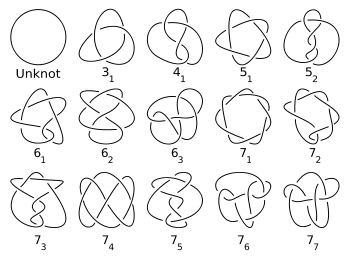
\includegraphics[width=\textwidth]{examples}
					\caption{Knots with $c(K)\leq 7$}
				\end{figure}
			\end{column}
			\hfill
			\begin{column}{.4\textwidth}
				\begin{figure}
					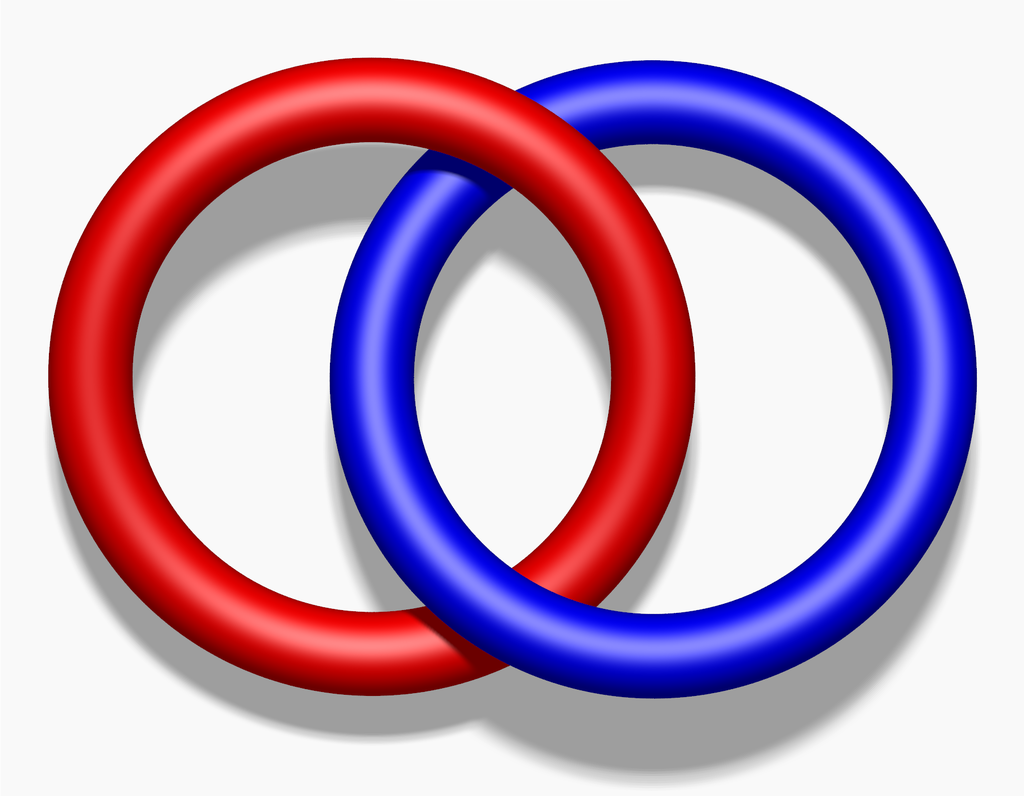
\includegraphics[width=\textwidth]{hopf}
					\caption{Hopf link}
				\end{figure}
			\end{column}
		\end{columns}
	\end{frame}

	\begin{frame}
		\frametitle{Reidemeister moves}
		
		\begin{theorem}[Reidemeister]
			Two knots $K,K'$ are isotopic if and only if they have diagrams that differ by a sequence of planar isotopies and Reidemeister moves.
		\end{theorem}
		
		\begin{center}
			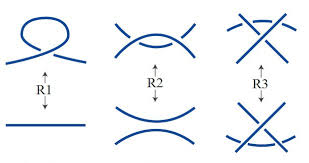
\includegraphics[scale=0.7]{reidemeister.jpg}
		\end{center}
	\end{frame}

	\begin{frame}
		\frametitle{Crossings}
		\begin{itemize}
			\item If we orient a knot $K$, then we can define a \textit{sign} for each crossing by the right-hand rule.
			
			\item For a two-component link $L=K\cup K'$, the \textit{linking number} $\lk(L)$ is one half the sum of the signs of the crossings between $K$ and $K'$ in a diagram of $L$.
		\end{itemize}
	
		\begin{center}
			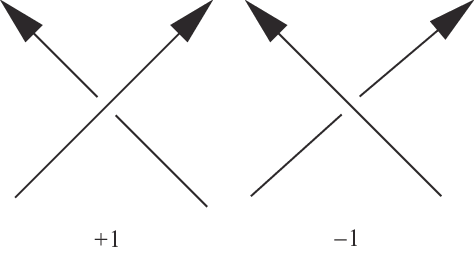
\includegraphics[scale=0.25]{signs}
		\end{center}
	\end{frame}

\begin{frame}
	\frametitle{Unknotting number and band move}
	\begin{definition}
		The \textit{unknotting number} $u(K)$ of a knot $K$ is the minimal number of crossing changes that are required to change some diagram of $K$ into a diagram of the unknot.
	\end{definition}
	\begin{itemize}
		\item If $u(K)$=0, then $K$ is an unknot.
	\end{itemize}
	\begin{definition}
		Let $K$ be any knot(or link) in $S^3$ and let $b \subset S^3$ be any embedded band where one pair of sides lie along arcs in $K$ and where $b$ is otherwise disjoint from $K$. Join $K$ to itself by deleting the arcs $K \cap b$ and adding the arcs forming the other side of $b$. The resulting knot(or link) $K'$ is obtained from $K$ by a \textit{band move} along $b$.
	\end{definition}
\end{frame}

\begin{frame}
	\frametitle{Example of band move and band presentation}
	\begin{itemize}
		\item Example of band move:
		
		The Stevedore knot $6_1$ is obtained from a band move on two unknots:
		\begin{figure}
			\hspace*{-1.5cm}\begin{center}{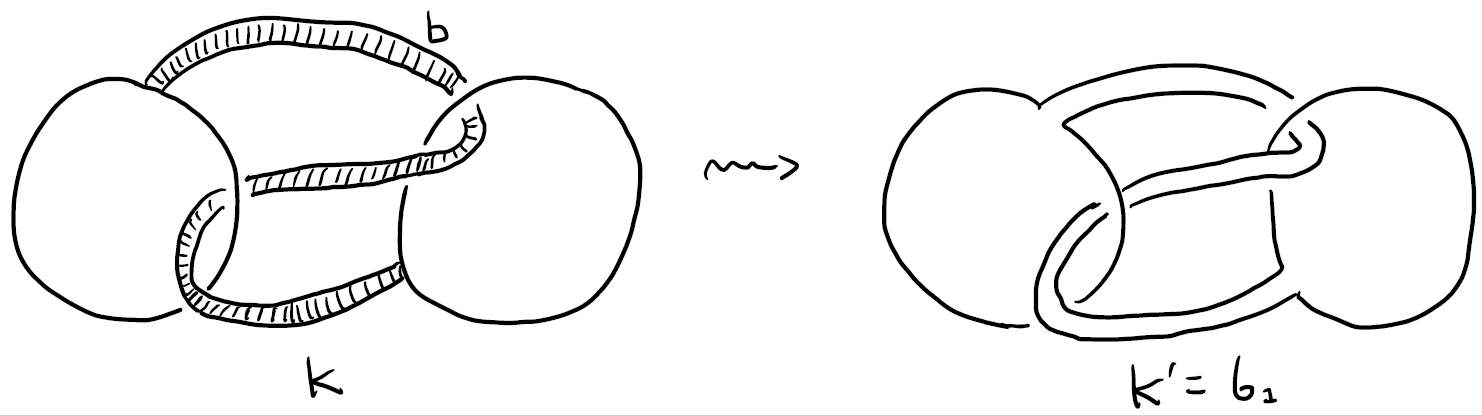
\includegraphics [width=8cm] {bandmove}}\end{center}
		\end{figure}
	\end{itemize}
	\begin{itemize}
		\item If $K$ can be obtained from another knot(or link) $K'$ by a single band move, then we say K has a \textit{band presentation}.
	\end{itemize}
	\begin{itemize}
		\item If $K$ can be obtained from a Hopf link by a single band move, then K has a \textit{banded Hopf link presentation}.
	\end{itemize}
\end{frame}

\begin{frame}
	\frametitle{Example of banded Hopf link presentation}
	\begin{theorem}
		If $K$ has $u(K)=1$, then it is obtained from the Hopf link by a single band move. 
	\end{theorem}
	\begin{itemize}
		\item Example: banded Hopf link presentation of Trefoil:
		\begin{figure}
			\begin{center}{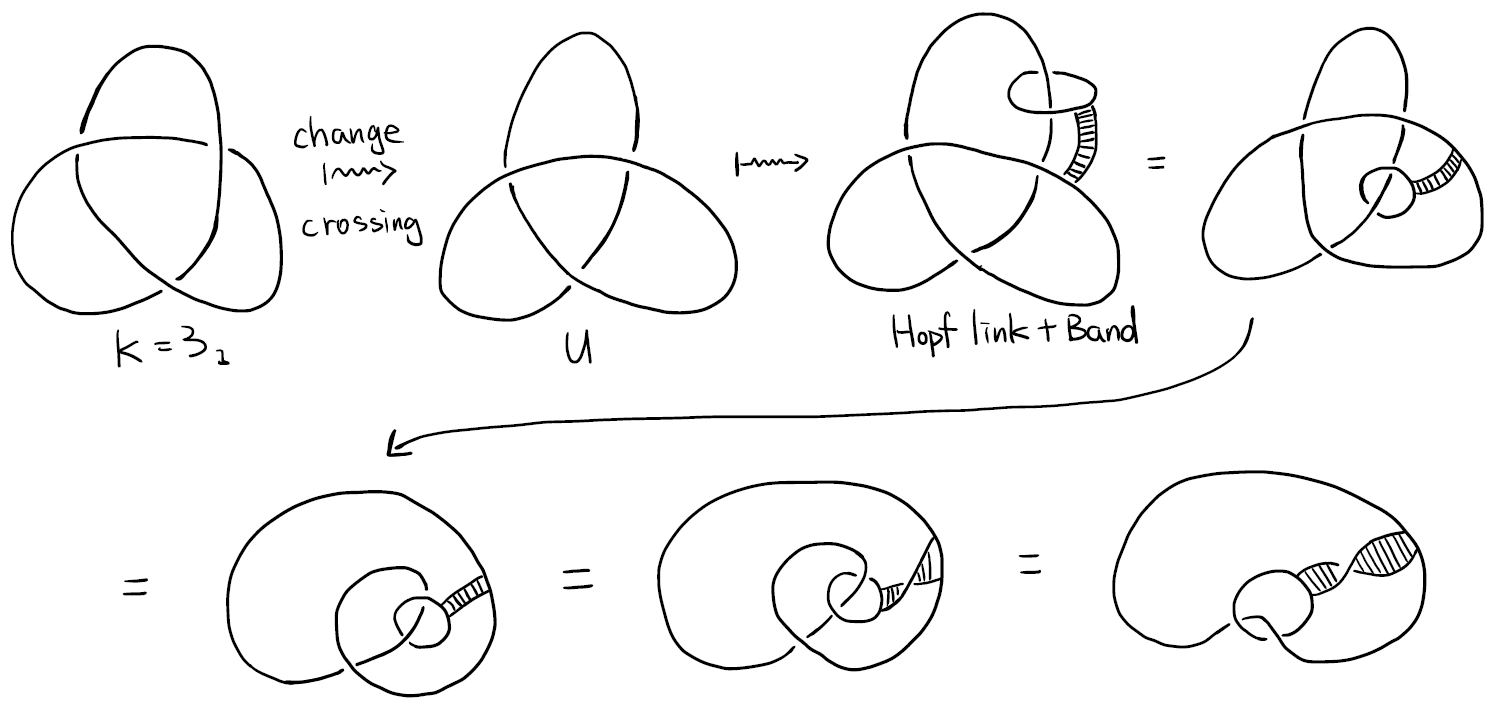
\includegraphics [width=10cm] {trefoil}}\end{center}
		\end{figure}
	\end{itemize}
\end{frame}

	\begin{frame}
		\frametitle{Twist knots and Twisted whitehead double}
		\begin{definition}
			A \textit{twist knot} $K$ is a knot obtained by repeatedly twisting an unknot and linking the ends together.
		\end{definition}
			\begin{figure}
				{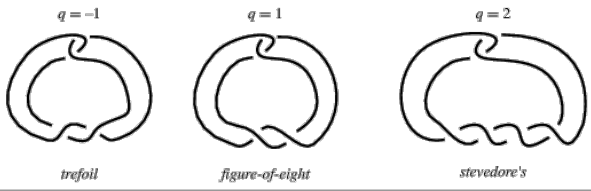
\includegraphics[scale=0.6] {twistknot}}
			\end{figure}
		\begin{definition}
			A knot $K$ is a \textit{twisted Whitehead double} if there exists a band presentation for K in which the band does not cross either component of the Hopf link. 
		\end{definition}
		\begin{itemize}
			\item Note: twist knots are twisted Whitehead doubles, but not all twisted Whitehead doubles are twist knots.
		\end{itemize}
	\end{frame}

	\begin{frame}
		\frametitle{Simple Closed Curves}
		\begin{definition}
			A \textit{simple closed curve} (s.c.c.) is a submanifold of a smooth manifold $X$, with itself diffeomorphic to $S^1$.
		\end{definition}
		\begin{figure}
			\centering
			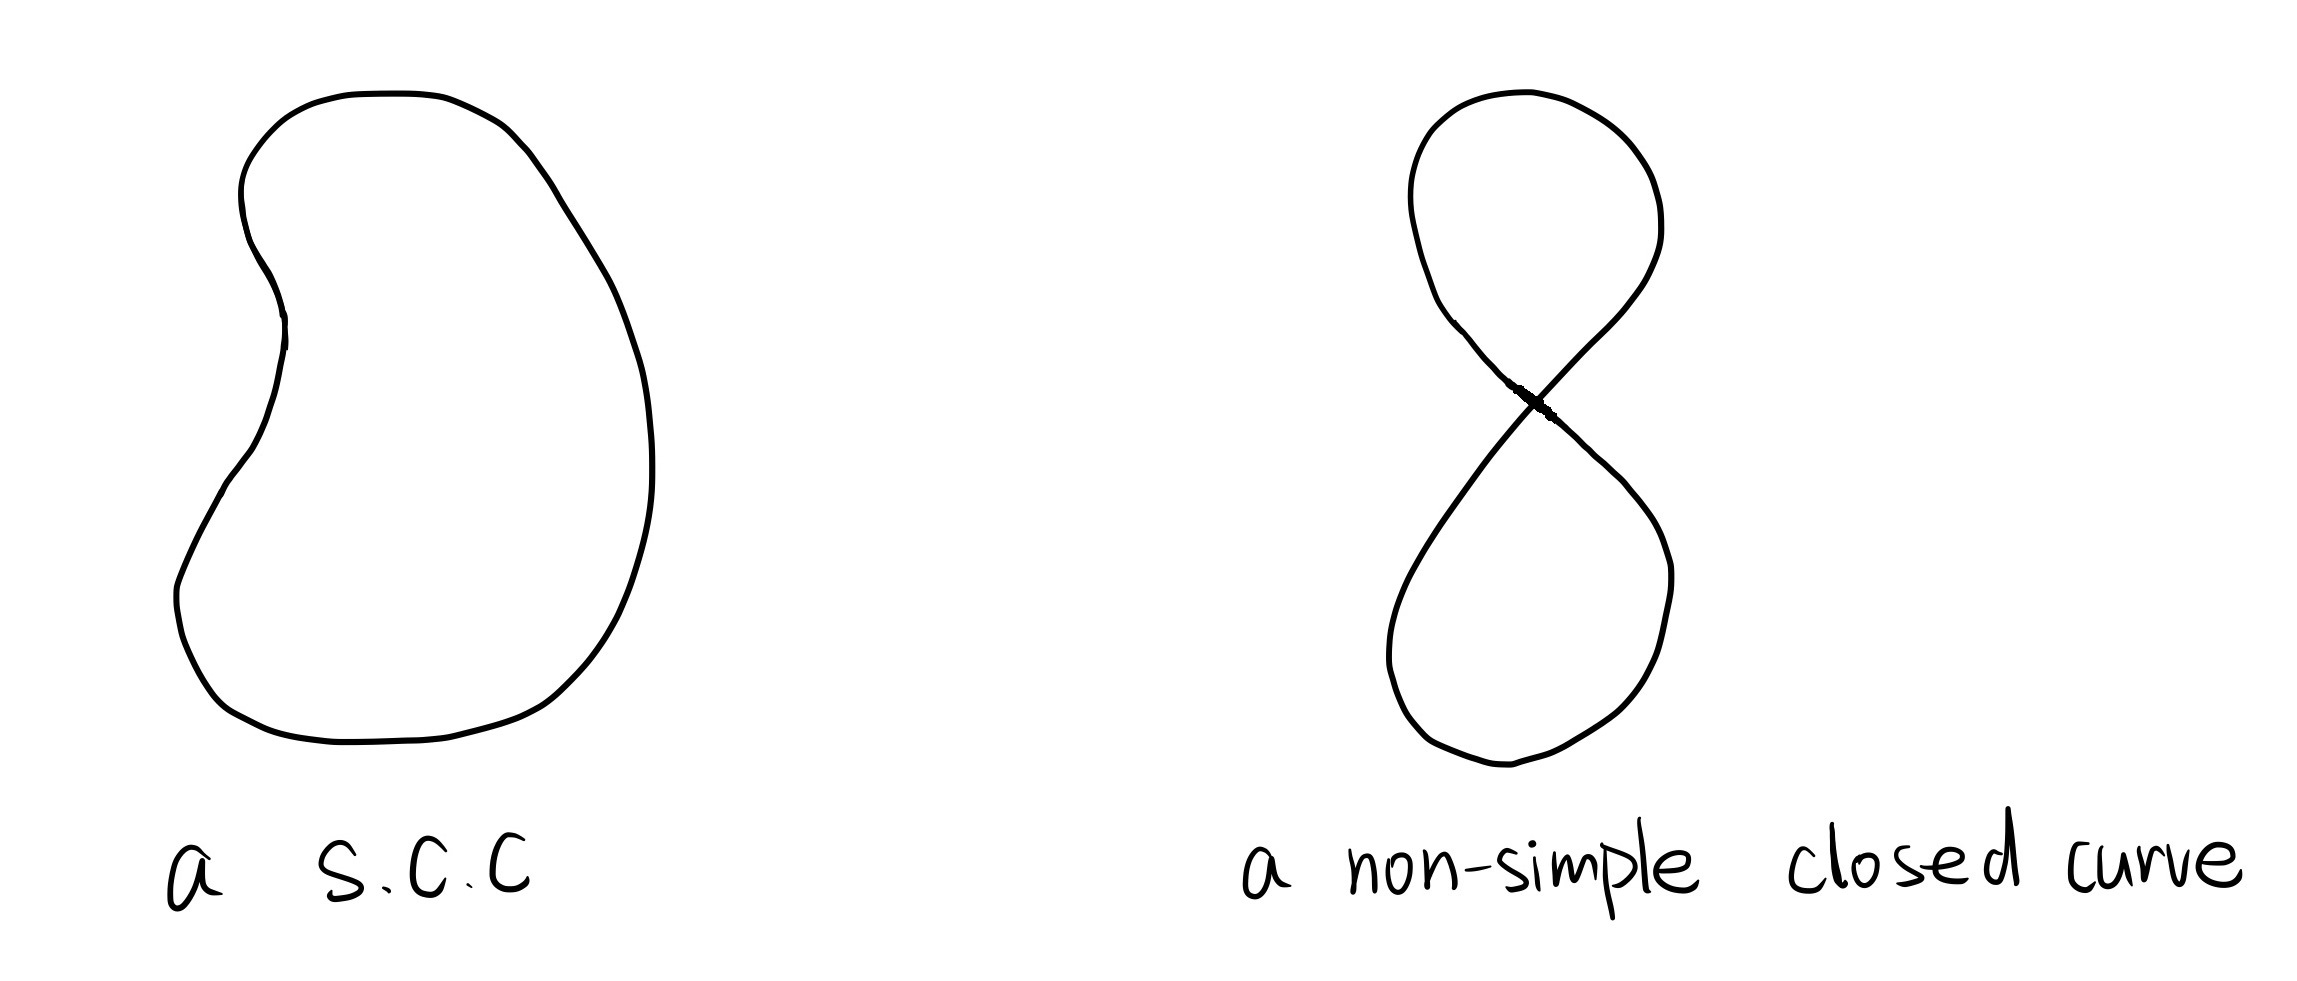
\includegraphics[width=50mm]{scc.jpg}
		\end{figure}
		\begin{itemize}
		\item By definition, a s.c.c. is embedded in some smooth manifold and is intuitively a $1$-dimensional curve diffeomorphic to $S^1$ without any self-intersection. 
		\item In particular, we can embed s.c.c.'s in a manifold such as a torus $T^2$. An alternate definition for a knot $K \subset S^3$ is a simple closed curve in $S^3$.
		\end{itemize}
	\end{frame}	

	\begin{frame}	
		\frametitle{Embedded s.c.c.'s on $T^2$}
		\begin{definition}
			A s.c.c. $\gamma \subset T^2$ is called \textit{non-separating} if $T^2-\gamma$ is connected.
		\end{definition}
		\begin{itemize}
		\item Every non-sperating s.c.c. in $T^2$ bounds a disc.
		\item Any two oriented and non-separating s.c.c's $\gamma, \gamma' \subset T^2$ are isotopic if and only if their signed intersection, the sum of their local intersections, is $0$.
		\end{itemize}
		\begin{definition} 
			Any two s.c.c.'s $\gamma, \gamma' \subset T^2$ form a \textit{basis} if they are non-separating and intersecting in a single point. 
		\end{definition}
		\begin{figure}
			\centering
			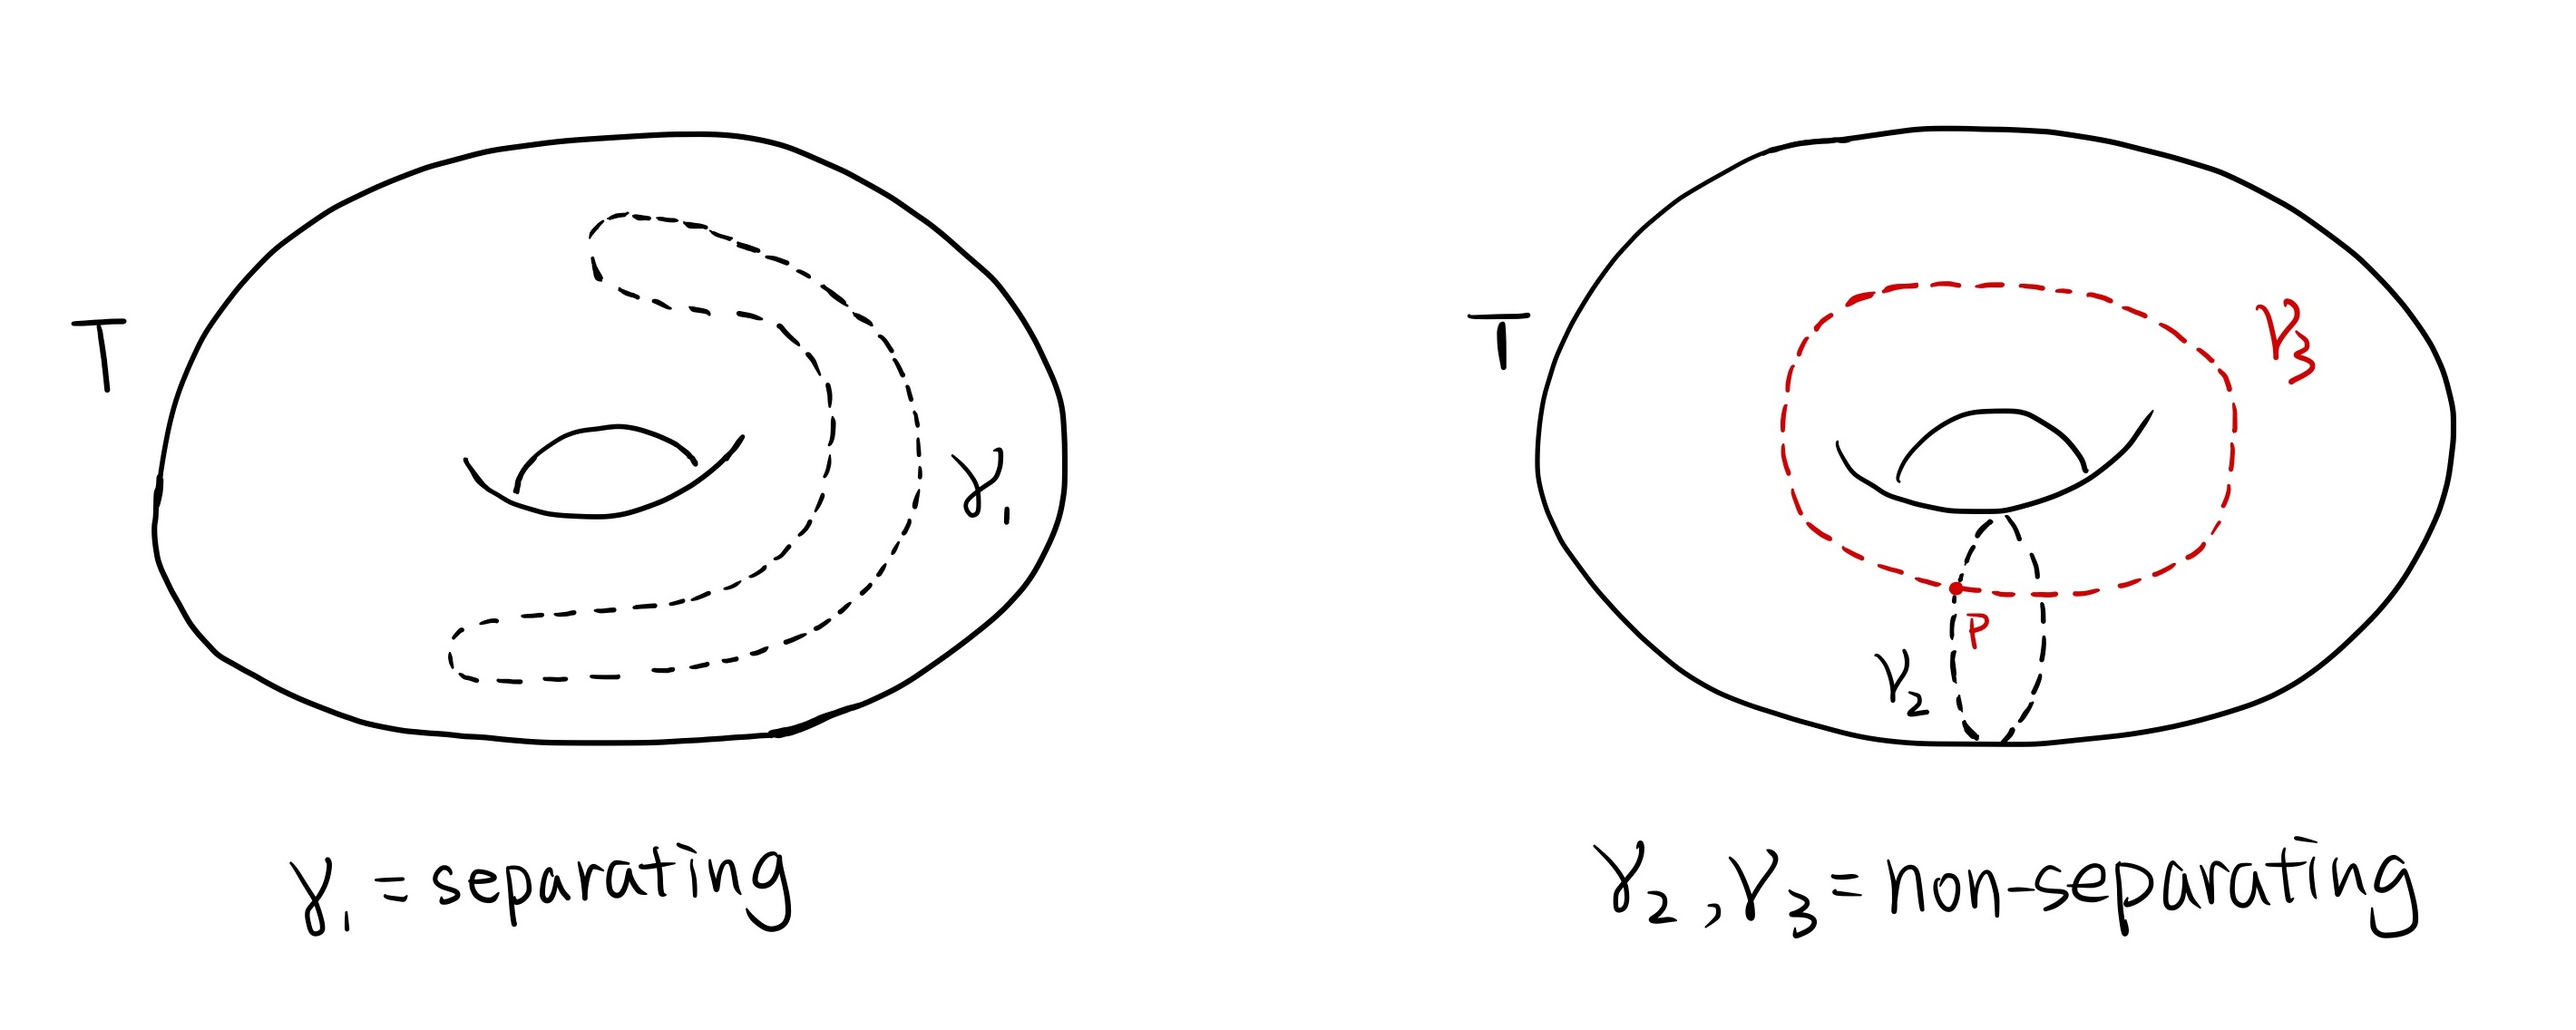
\includegraphics[width=60mm]{Separating.jpg}
		\end{figure}
	\end{frame}

	\begin{frame}
		\frametitle{Preferred meridian and longitude pair for a knot $K \subset S^3$}
		\begin{definition} 
		Given a knot $K \subset S^3$, $N(K) \cong S^1 \times D^2 \cong$ a solid torus $\mathbb{T}$ where $\partial N(K) \cong$ a torus $T^2$, we define a \textit{meridian} $\mu$ of $K$ to be an unknot $\partial D^2 \times {1} \subset \partial N(K) \cong T^2$ that bounds a disc which $K$ crosses exactly once. Then we choose a longitude of $K$ as a circle $\lambda = {1} \times S^1 \subset \partial N(K) \cong T^2$, which is a parallel copy of $K$ on $\partial N(K)$.
		\end{definition}
		\begin{figure}
			\centering
			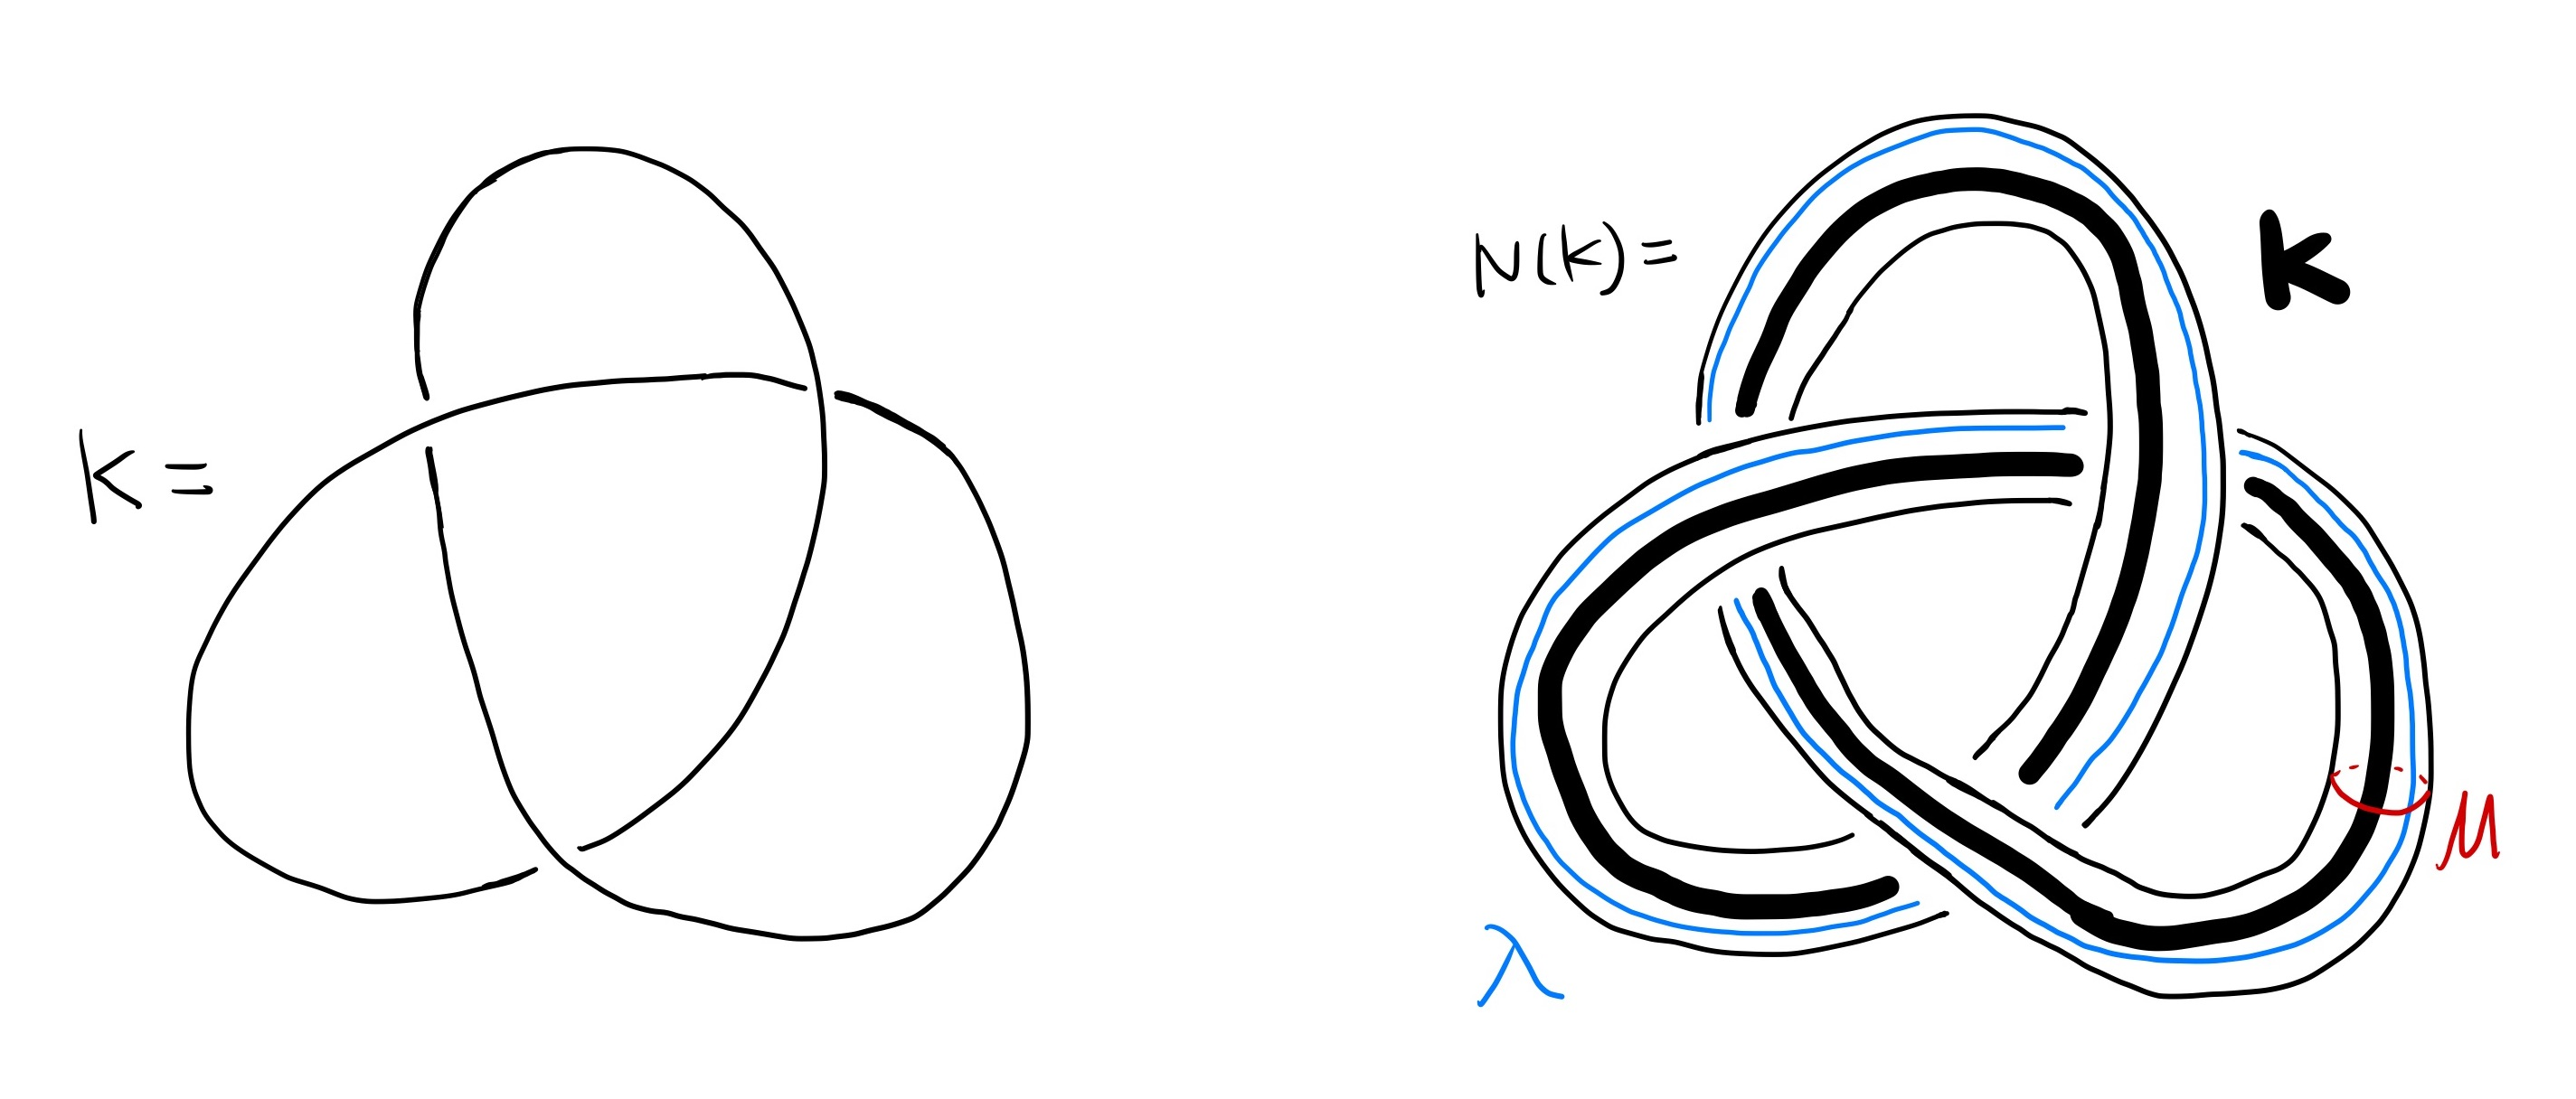
\includegraphics[width=60mm]{N(K).jpg}
		\end{figure}
		\begin{itemize}
		\item Note that our choice of the longitude $\lambda$ for $K$ intersects the meridian $\mu$ non-tangentially in exactly one point, and thus ($\mu, \lambda$) form a basis of $T^2$.
		\end{itemize}
	\end{frame}	

	\begin{frame}
		\frametitle{Isotopy classes of s.c.c.'s on $T^2$}
		\begin{itemize}
		\item If a preferred basis of a torus $T^2$ is $(m, l)$, then any s.c.c $\gamma \subset T^2$ can be determined (up to isotopy) by two numbers, $p:=|n(\gamma \cap m)|$ and $q:=|n(\gamma \cap l)|$ where $n(a \cap b)$ is the signed intersection between the two oriented simple closed curves $a$ and $b$ on $T^2$. 
		\end{itemize}
		\begin{itemize}
		\item Further, isotopy classes s.c.c's on a torus are classified by the set of extended rational numbers $\mathbb{Q}\cup\{\infty\}$. 
		\end{itemize}		
		\begin{itemize}
		\item Hence, given a knot $K \in S^3$ where $\partial N(K) \cong$ a torus $T^2$, any $p/q \in \mathbb{Q}\cup\{\infty\}$ determines a s.c.c $\beta$ on $\partial N(K)$ that is well-defined up to isotopy. Intuitively, $p$ (and $q$ resp.) is the number of of times that $\beta$ goes around the meridian (and longitude resp.) that we choose for $K$. 
		\item We use $\beta$ to define a $3$-manifold $S^3_{p/q}(K)$, called $p/q$-surgery on $K$.
		\end{itemize}
	\end{frame}

	\begin{frame}
		\frametitle{Surgery on a knot: \textit{drilling} then \textit{filling}}
		\begin{definition}
		Given a knot $K \subset S^3$, the \textit{exterior} of $K$, denoted $X(K)$, is a manifold with boundary obtained by removing the interior of $N(K) = S^1 \times D^2 \cong$ a solid torus $\mathbb{T}$ from $S^3$. Then $\partial X(K) = \partial N(K) \cong$ a torus $T^2$. Let $\beta$ be the s.c.c on $T^2$ determined (up to isotopy) by some extended rational number $p/q \in \mathbb{Q}\cup\{\infty\}$. Then the \textit{$p/q$-surgery} on $K$, a $3$-manifold denoted $S^3_{p/q}(K)$, is obtained by gluing another solid torus $\mathbb{T'}$ back to $X(K)$ so that the meridian of $\mathbb{T'}$ is identified with the curve $\beta$. 
		\end{definition}
	\end{frame}

	\begin{frame}
	\frametitle{Examples of $p/q$-surgery on a knot}
		\begin{itemize}
		\item Example: $\pm 1/0$-surgery on a knot $K$ gives back $S^3$ trivially. Thus any nontrivial surgery on a knot $K$ has rational slopes.  			
		\end{itemize}
		\begin{itemize}
		\item Example: $S^3_{1/n}(u) \cong S^3$ where $u$ is an unknot and $n \in \mathbb{Z}$.
		\end{itemize}
		\begin{figure}
			\centering
			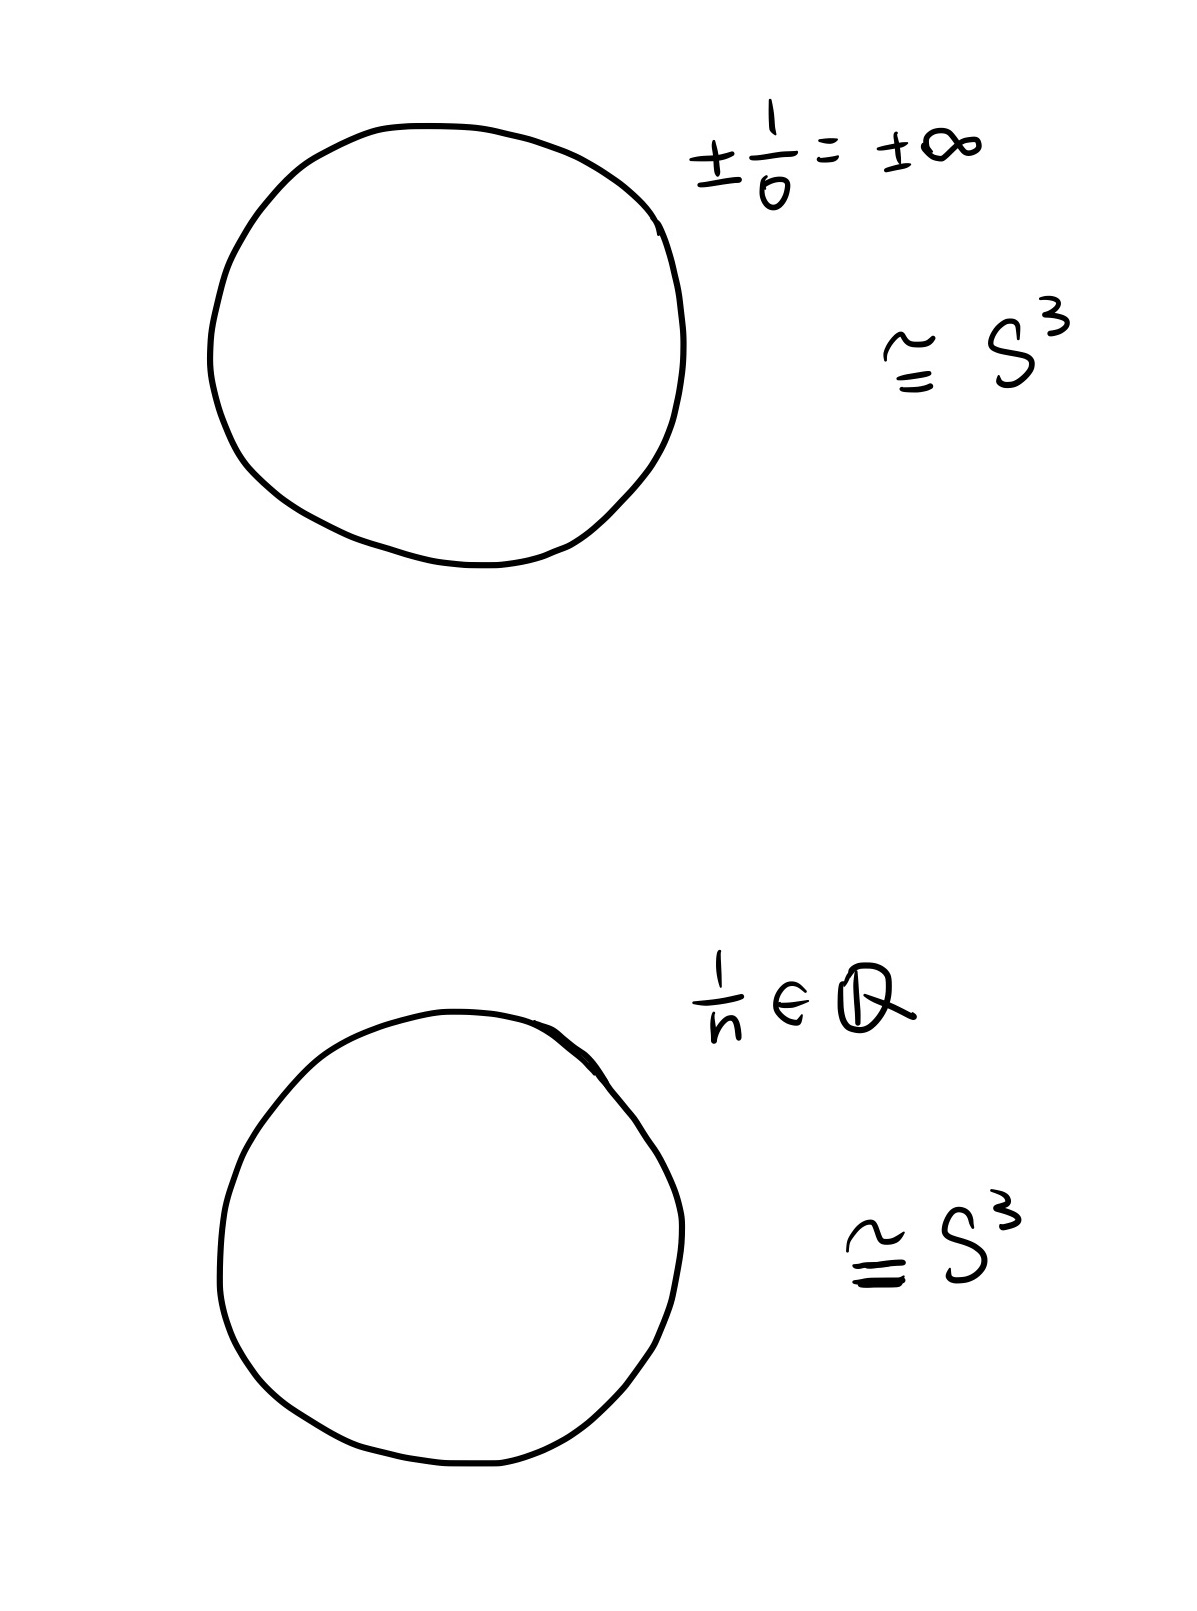
\includegraphics[width=30mm]{Unknot.jpg}
		\end{figure}	
	\end{frame}

	\begin{frame}
	\frametitle{Surgery on a link}
		\begin{definition}
		Similarly, given a link $L$ in $S^3$ s.t. $\exists p/q \in \mathbb{Q}\cup\{\infty\}$ associated to each component of $L$, we can do surgery on $L$ by doing surgery along each of its component. Any such link is called a \textit{framed} link. 
		\end{definition}
	\begin{itemize}
		\item Example: for any integer $n$, $(n, 0)$-surgery on a Hopf link $K$ yields $S^3$.
	\end{itemize}
	\begin{figure}
		\centering
		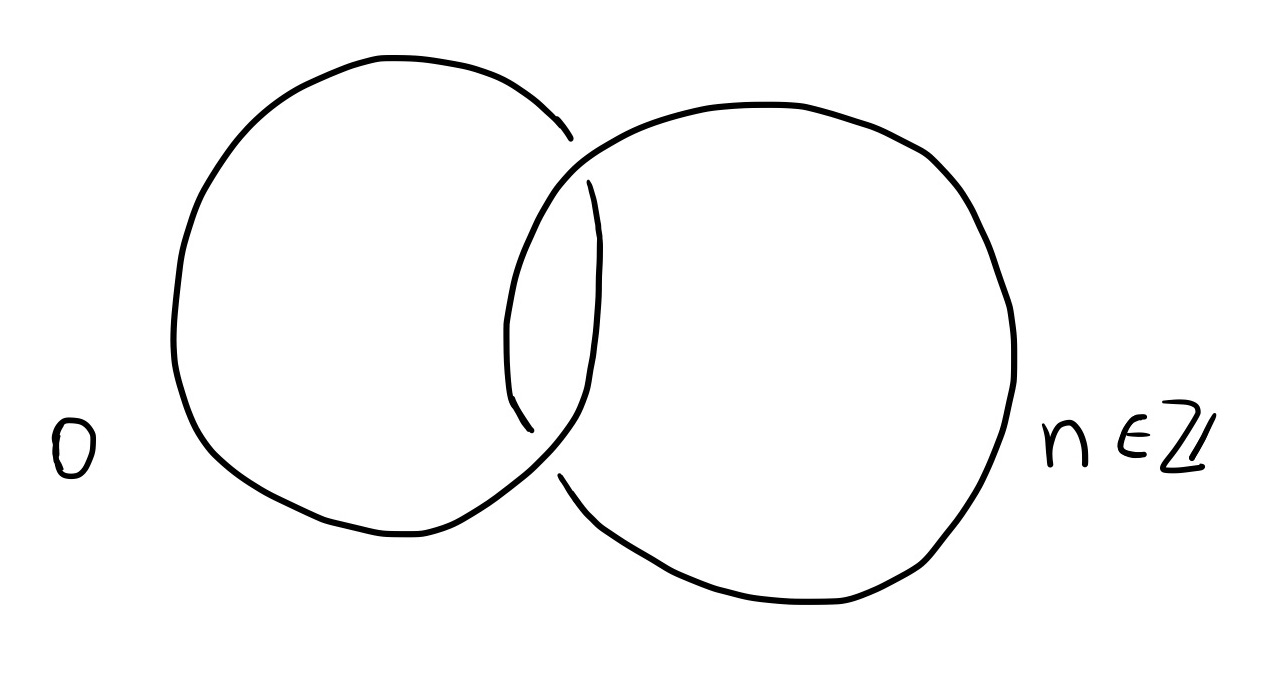
\includegraphics[width=30mm]{Hopf.jpg}
	\end{figure}
		\begin{theorem}
		Any oriented, connected $3$-manifold can be obtained by doing surgery along a framed link. So we can think of any $3$-manifold in terms of a diagram for a framed link. Any such diagram is called a \textit{surgery diagram}. 
		\end{theorem}
		
	\end{frame}

	\begin{frame}
	\frametitle{Example of surgery on a link}
		\begin{theorem}
		For any integer $n$ and any knot $K$ with an unknot $c$ as its meridian, $(n, 0)$-surgery on $K \cup c$ yields $S^3$. Such a pair of $K$ and $c$ forms a cancelling pair that can be deleted without changing the $3$-manifold described by the surgery diagram.
		\end{theorem}
		\begin{figure}
			\centering
			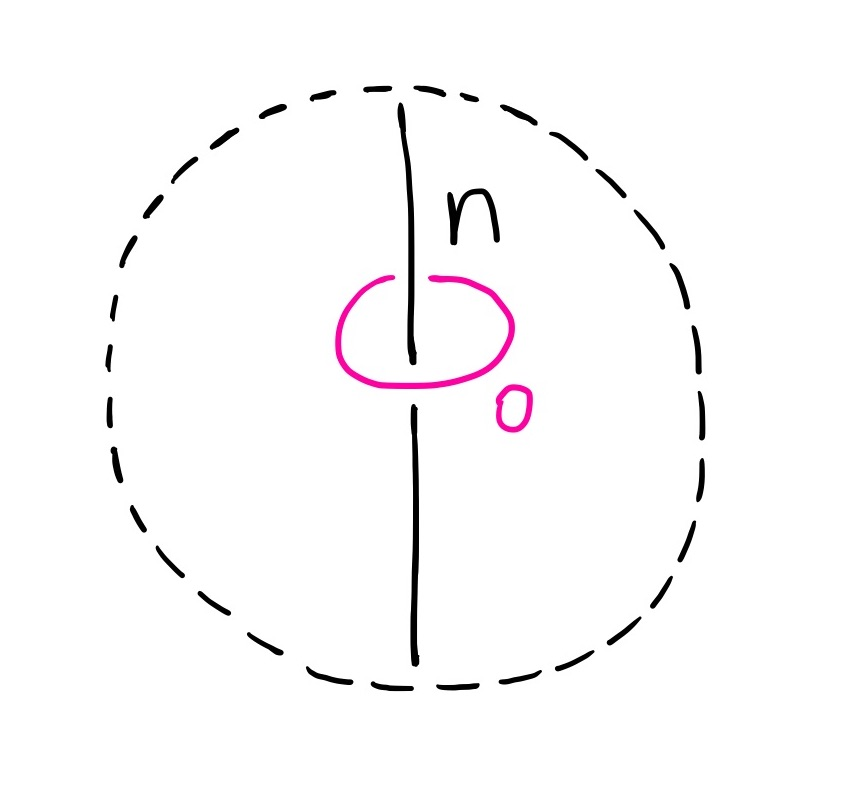
\includegraphics[width=50mm]{Kc.jpg}
		\end{figure}
	\end{frame}

	\begin{frame}
	\frametitle{Surgery dual to a knot}
		\begin{itemize}
		\item Note that $K$ is given by $S^1 \times {0}$ inside $N(K) = S^1 \times D^2 \cong$ a solid torus $\mathbb{T}$. i.e. $K$ is the core curve of the solid torus $N(K)$. 
		\end{itemize}
		\begin{figure}
			\centering
			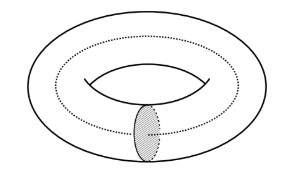
\includegraphics[width=30mm]{core.png}
		\end{figure}
		\begin{definition}
		When doing $p/q$-surgery on a knot $K \in S^3$, the new solid torus $\mathbb{T'} \cong S^1 \times D^2$ that we glue back in $X(K)$ to produce $S^3_{p/q}(K)$ also has a core curve $S^1 \times {0}$, which specifies a knot $\gamma$ in $S^3_{p/q}(K)$. Call $\gamma$ the \textit{surgery dual} of $K$.
		\end{definition}		
	\end{frame}

	\begin{frame}
	\frametitle{Surgery dual to a knot (cont.)}
		\begin{itemize} 
		\item For any knot $K$ and any integer $n$, the \textit{surgery dual} to $K$ in $S^3_n(K)$ can be represented as a meridian to $K$ in the surgery diagram. 
		\end{itemize}
		\begin{figure}
			\centering
			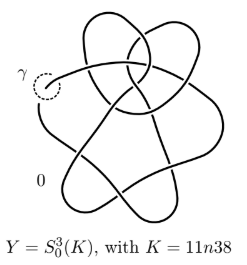
\includegraphics[width=25mm]{dual.png}
		\end{figure}
		\begin{lemma}
		Surgery duality for knots in $S^3$ is symmetric. 
		\end{lemma}
		\begin{figure}
			\centering
			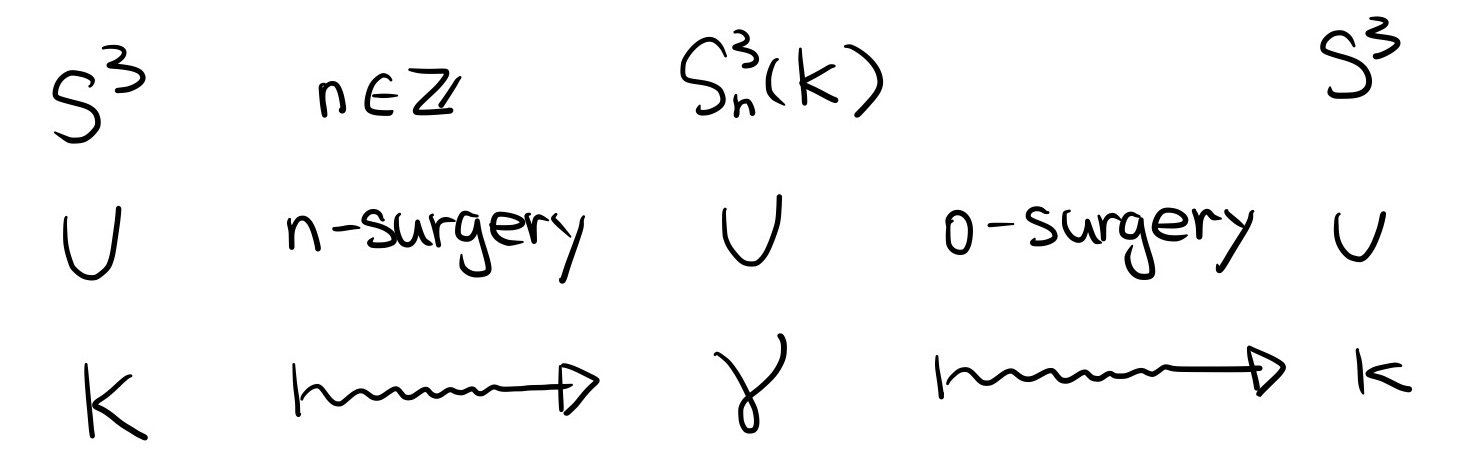
\includegraphics[width=50mm]{Symmetry.jpg}
		\end{figure}
	\end{frame}

	\begin{frame}
	\frametitle{Surgery dual link to a framed link}
		\begin{definition}
		A \textit{surgery dual link} to a framed link $L=\bigcup^{N}_{i=1} L_i \in S^3$ is a link $L' = \bigcup^{N}_{i=1} L'_i$, where each component $L'_i$ is the surgery dual to $L_i$ in the surgered manifold $Y$ that we obtain after doing surgery on $L$.
		\end{definition}
	\end{frame}
	
	%mark of my intro part, where Anton should introduce next Kirby Calculus and integral vs. rational surgery


	\begin{frame}
	\frametitle{Piccirillo's construction: Knots with the same surgery}
	\begin{theorem}[Piccirillo 2018]
		Let $L = R \cup G \cup B$ be a surgery diagram for some 3-manifold $Y$ such that:
		\begin{enumerate}
			\item $R$ is a zero-framed unknot, $B$ and $G$ have integral framings.
			\item Ignoring $B$, $R$ is isotopic to a meridian of $G$.
			\item Ignoring $G$, $R$ is isotopic to a meridian of $B$.
			\item $B$ and $G$ have linking number $0$.
		\end{enumerate}
		Then, there exist knots $K$ and $K'$ such that $Y \cong S^3_{n}(K) \cong S^3_{n}(K')$.
	\end{theorem}
	\begin{itemize}
		\item Piccirillo's construction comes from an older construction, the \textit{dualizable patterns} construction, to produce knots with the same surgery.
	\end{itemize}
\end{frame}

\begin{frame}
	\frametitle{Piccirillo's construction (cont.)}
	\begin{figure}
		\begin{center}
			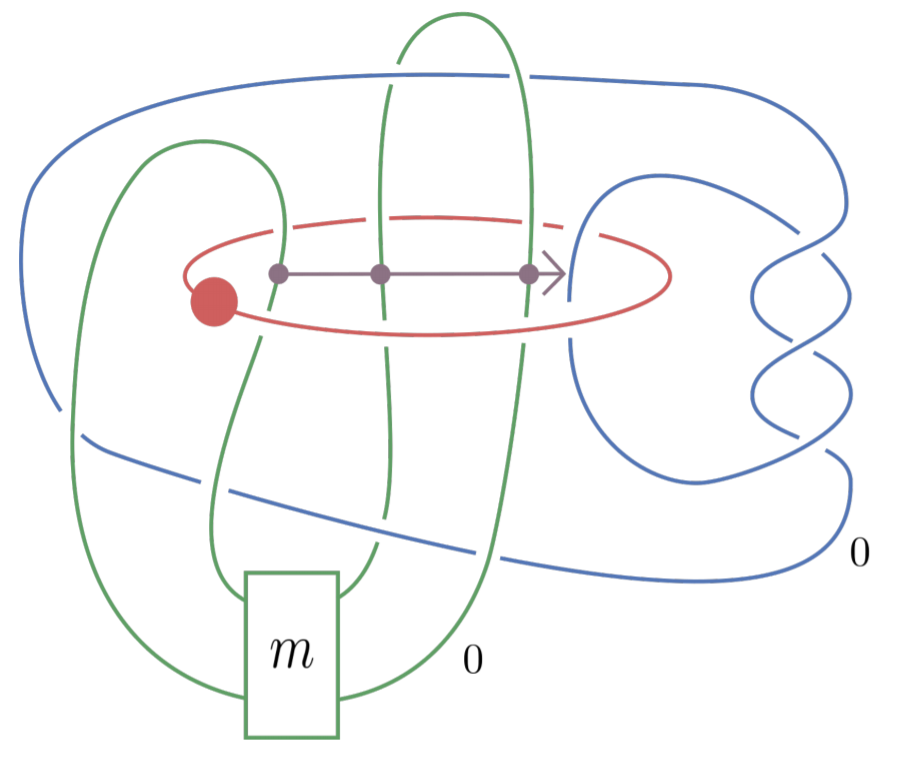
\includegraphics[width=3in]{picci.png}
			\caption{Diagram of a link $L$ used by Piccirillo on her original paper. The colors (red, blue, and green) match the component letters $R$, $B$, $G$.}
		\end{center}
	\end{figure}
\end{frame}


	\begin{frame}
		\frametitle{Baker-Motegi: Knots with the same surgery}
			\begin{itemize}
				\item We adapted the following construction from Baker and Motegi (2018).
				
				\item Let $K$ be a knot, and suppose we can take an unknot $c$ linked with $K$ such that $(0,0)$-surgery on $K\cup c$ is $S^3$.
				
				\item Baker-Motegi present a method for producing knots $K_n'$ with $S^3_n(K)\cong S^3_n(K_n')$ from this link.
				
				\item Define $K'$ to be the surgery dual to $c$ in $S^3=S^3_{(0,0)}(K\cup c)$.
				
				\item Then $K'$ has the same 0-surgery as $K$.
				
			\end{itemize}
		
			
	
	\end{frame}

	\begin{frame}
		\frametitle{Baker-Motegi (cont.)}
		\begin{itemize}
			
			\item Also define $c'$ to be the surgery dual to $K$ in $S^3$.
			
			\item After some Kirby calculus, we find that in the surgered manifold $S^3=S^3_{(0,0)}(K\cup c)$, $c'$ is an unknot linked with $K'$.
			
			\item Let $K_n'$ be the result of twisting $K'$ through $c'$, $n$ times.
			
			\item We say that $\{K_n'\}$ forms a \textit{twist family}.
			
			\item Then $K_n'$ has the same $n$-surgery as $K$ for all $n$.
			
			\item Moreover, if $c$ is not a meridian to $K$, then $K\simeq K_n'$ for at most finitely many $n$.
		\end{itemize}
	\end{frame}

	\begin{frame}
		\frametitle{Baker-Motegi Illustration}
		\begin{center}
			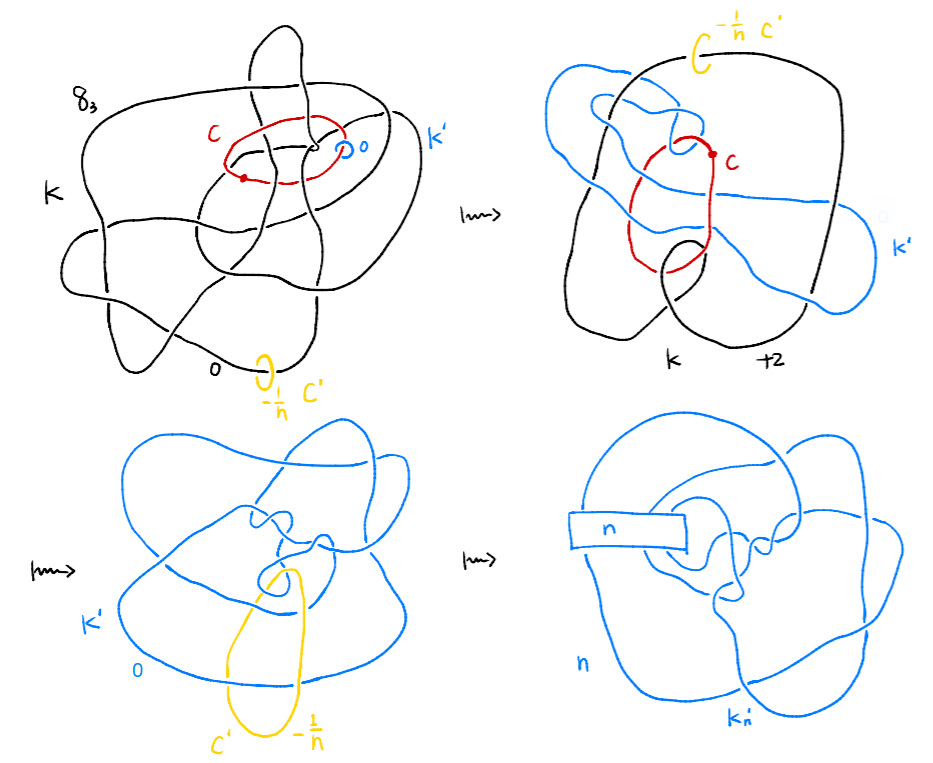
\includegraphics[scale=0.5]{bm}
		\end{center}
	\end{frame}

	\begin{frame}
		\frametitle{Obtaining a link $K\cup c$ when $u(K)=1$ (Piccirillo)}
		\begin{itemize}
			\item In the special case where $K$ has unknotting number one, we can use a band presentation for $K$.
			
			\item We start with a Hopf link $R\cup B$ and slide one component over the other according to the band presentation for $K$.
			
			\item $R$ remains an unknot, which we rename $c$, and $B$ becomes $K$.
			
			\begin{lemma}
				Let $K\cup c$ be the link obtained by the handle slide above. Then $(0,0)$-surgery on $K\cup c$ gives $S^3$.
			\end{lemma}
			
			\begin{center}
				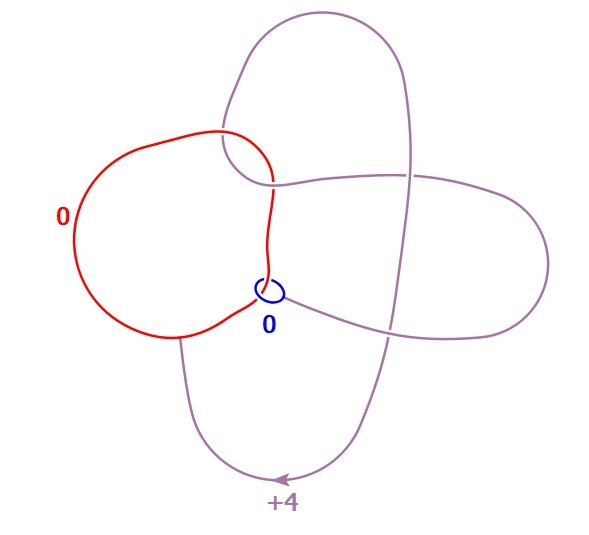
\includegraphics[scale=0.4]{k_cup_c_example1}
				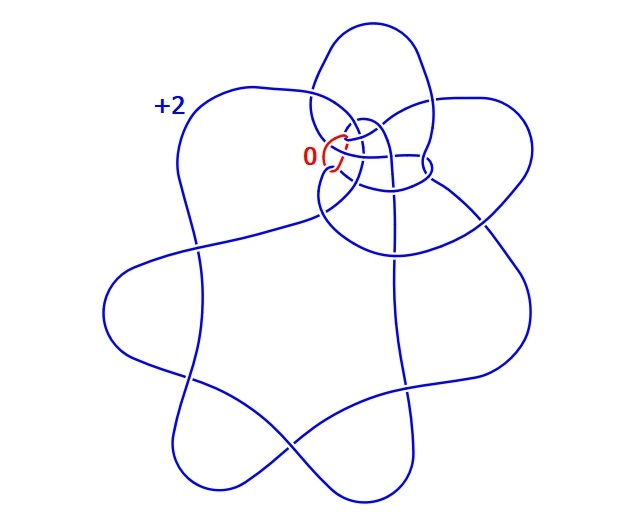
\includegraphics[scale=0.4]{k_cup_c_example2}
			\end{center}
		\end{itemize}
	\end{frame}

	

	\begin{frame}
		\frametitle{Obtaining $K\cup c$ when $u(K)>1$}
		
		\begin{itemize}
			\item We do not have a systematic way of finding a link $K\cup c$ for a given knot $K$ with $u(K)>1$.
			
			\item If we perform multiple slides on a Hopf link, then we obtain a link $K\cup c$ for some knot $K$ with higher unknotting number, but we have no way of predicting what $K$ will be.
			
			\item Example: $10_{125}$
			
			\begin{center}
				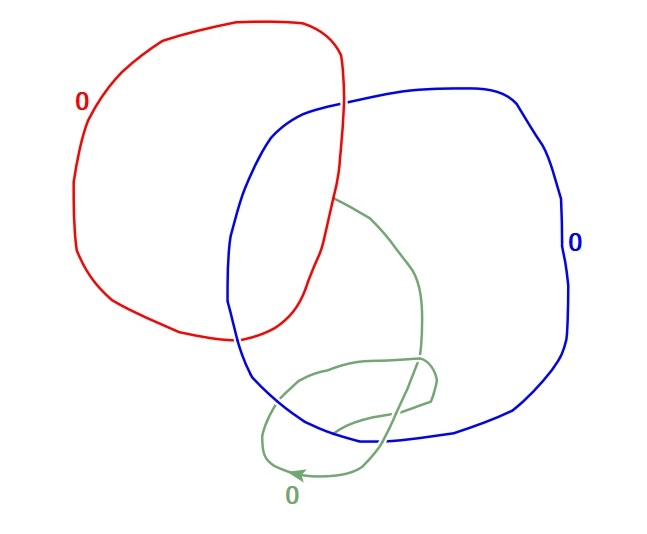
\includegraphics[scale=0.25]{10_125_1}
				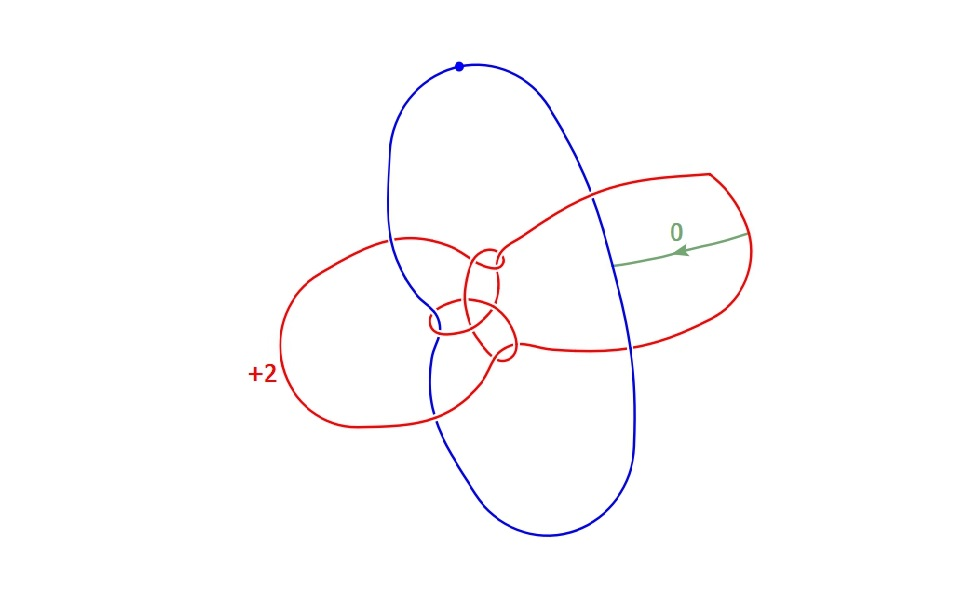
\includegraphics[scale=0.25]{10_125_2}
				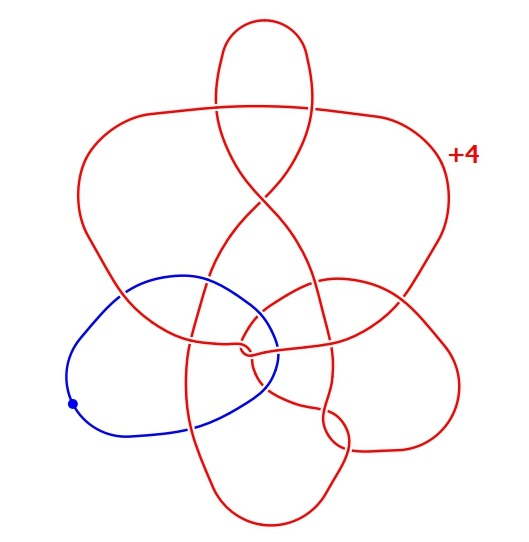
\includegraphics[scale=0.25]{10_125_3}
			\end{center}
		\end{itemize}
	\end{frame}

\begin{frame}
	\frametitle{Applications of the construction}
	\begin{itemize}
		\item We have produced a banded Hopf link presentation for all the 78 unknotting number one knots $K$ with $c(K)\leq 10$.
		\item We followed the above procedure to manually produce a diagram for a knot $K'$ that has the same zero-surgery as $K$, using a software called KLO which can perform Kirby calculus on link diagrams.
		\item Using a software called SnapPy, we were able to verify that whenever $K$ was not a twist knot, $K'$ was not isotopic to $K$. Thus, zero was not a characterizing slope.
		\item We can use a similar process to check whether any integer slope is characterizing.
	\end{itemize}
	\medskip
	\begin{itemize}
		\item \textbf{Question:} Can we classify all integer slopes once we have the link $K\cup c$, with finitely many computations?
	\end{itemize}
\end{frame}


	\begin{frame}
	\frametitle{Ruling Out Integer Characterizing Slopes}
	\begin{itemize}
		\item We developed an algorithm that can be carried out by a computer script to rule out the integer characterizing slopes of some knot $K$, once we have manually produced the link $L = K \cup c$.
	\end{itemize}
	\begin{enumerate}
		\item Given a link $L$, run SnapPy commands to find out the volume of the knot $K$, the volume of the manifold $Z = S_0^3(c)$, and the length of the Seifert longitude in $Z$.
		\item Using these values, apply the theorems of hyperbolic Dehn surgery to find the bound $N$ such that any integer $|n| > N$ is a characterizing slope for $K$.
		\item  For the remaining $2N + 1$ cases, verify if the volume of the knot with the same $n$-surgery as $K$ matches the volume of $K$.
	\end{enumerate}
	\begin{itemize}
		\item We use the \textit{DT code} of the link, which uniquely describes all links that we deal with, up to isotopy.
	\end{itemize}
\end{frame}

\begin{frame}
\frametitle{Findings}
\begin{theorem}[Low-Crossing Knots]
	Regarding the integer slopes of knots $K$ such that $c(K) \leq 10$:
	\begin{itemize}
		\item If $K$ has unknotting number $u(K) = 1$ and $K$ is not a twist knot, then $K$ has at most \textit{one} integer characterizing slope, namely $\pm 2$.
		\item If $K$ is the twist knot $8_1$, then $K$ has at most \textit{one} integer characterizing slope, namely $0$.
		\item If $K$ is one of the $u(K) = 2$ knots $8_4$, $8_6$, $8_{10}$, $8_{12}$, $8_{16}$, $10_{148}$, $10_{149}$, or $10_{150}$, $K$ has no possible integer characterizing slope.
		\item If $K$ is one of the $u(K) = 2$ knots $8_3$, $10_{125}$, or $10_{126}$, $K$ has at most \textit{one} integer characterizing slope.
	\end{itemize}
\end{theorem}
\end{frame}

	\begin{frame}
		\frametitle{Main theorem}
		\begin{theorem}
			If a knot $K$ has unknotting number $u(K)=1$ and is not a twisted Whitehead double, then $K$ has at most finitely many integer characterizing slopes.
		\end{theorem}
	\end{frame}

	\begin{frame}
		\frametitle{Proof of theorem}
		\begin{proposition}
			Let $K$ be a knot in $S^3$. Suppose we can take an unknot $c$ linked with $K$ so that $(0,0)$-surgery on $K\cup c$ yields $S^3$ and $c$ is not a meridian of $K$. Then $K$ has at most finitely many integer characterizing slopes.
		\end{proposition}
		\begin{itemize}
			\item This is a strengthened form of a result proven by Baker-Motegi, which we proved using symmetry of surgical duality.
		\end{itemize}
	\end{frame}


	\begin{frame}
		\frametitle{Proof of theorem (cont.)}
		\begin{itemize}
			\item Recall that  for $K$ with $u(K)=1$, we could obtain a link $K\cup c$ as in Baker-Motegi with $(0,0)$-surgery $S^3$ by sliding over a Hopf link according to the band presentation for $K$.
			
			\item It remains to show that if $K$ is not a twisted Whitehead double, then $c$ is not a meridian to $K$ after the handle slide.
			
			\item In this case, in any band presentation for $K$, the band must cross the disc bounded by one of the components of the Hopf link.
			
		\end{itemize}
	
		\begin{lemma}
			Let $R\cup B$ be a Hopf link, and consider a handle slide of $R$ over $B$ yielding a link $L$ in which $R$ remains a meridian to $B$. Then there exists a handle slide of $R$ over $B$, yielding a link isotopic to $L$, along a band that does not cross either of the discs bounded by $R$ or $B$.
		\end{lemma}
	\end{frame}

\begin{frame}
	\frametitle{Extension of theorem}
	\begin{itemize}
		\item How can we drop the condition on twisted Whitehead doubles? And on unknotting number?
		\item Can we produce an algorithm to find links $L = K \cup c$ from handle slides on a Hopf link?
	\end{itemize}
	\begin{conjecture}
		If $K$ is a knot with unknotting number $u(K) = 1$ and $K$ is not a twist knot, then $K$ has at most \textit{one} integer characterizing slope: $\pm 2$.
	\end{conjecture}
\end{frame}

\begin{frame}
	\frametitle{Next Steps}
	\begin{itemize}
		\item Rigorously prove the lemma on band presentations.
		\item Keep experimenting with handle slides in order to expand the list on Theorem 1.2.
		\item Attempt to use other tools to prove a version of Theorem 1.1 for Twisted Whitehead Doubles.
		\item Look into our final conjecture.
	\end{itemize}
\end{frame}


\end{document}

